% !Mode:: "TeX:UTF-8"	% read in as utf8 file.

\chapter{Plate}

\section{Constant strain triangle}
When a flat plate is subjected to both inplane and transverse or normal loads as shown
in Figure \ref{fig: inplane transverse loads in plane} any point inside the plate can have displacement components $ u, v $, and
$ w $ parallel to $ x, y $, and $ z $ axes, respectively. In the small deflection (or linear) theory of thin plates, the transverse deflection $ w $ is uncoupled from the inplane deflections u and v. Consequently, the stiffness matrices for the inplane and transverse deflections are also uncoupled and they can be calculated independently. Thus, if a plate is subjected to inplane loads only, it will undergo deformation in its plane only. In this case, the plate is said to be under the action of "membrane" forces. Similarly, if the plate is subjected to transverse loads (and/or bending moments), any point inside the plate experiences
essentially a lateral displacement $ w $ (inplane displacements $ u $ and $ v $, are also experienced because of the rotation of the plate element). In this case. the plate is said to be under the action of bending forces. The inplane and bending analysis of plates is considered in this chapter. If the plate elements are used for the analysis of three-dimensional structures. such as folded plate structures, both inplane and bending actions have to be considered in the development of element properties. This aspect of coupling the membrane and bending actions of a plate element is also considered in this chapter.

\begin{figure}[h!]
\centering
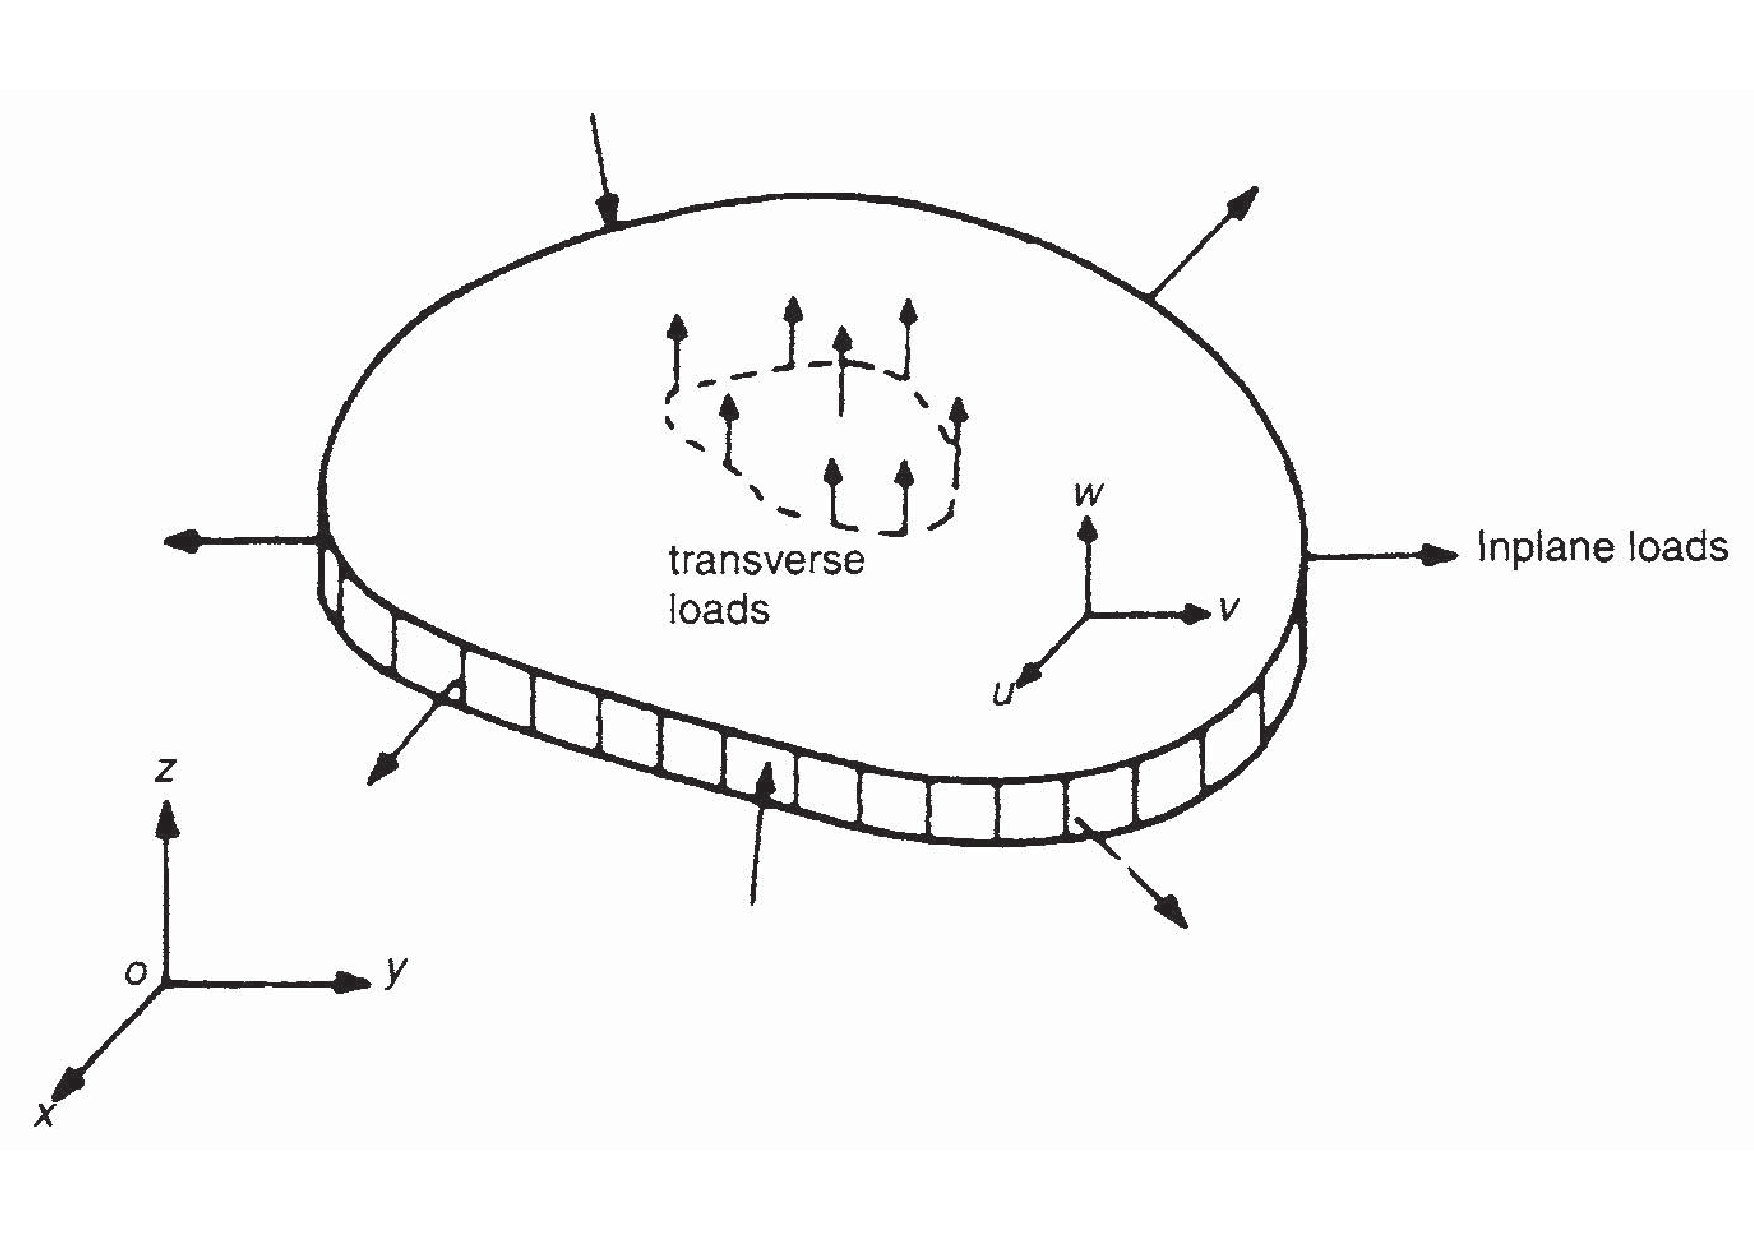
\includegraphics[width=0.5\linewidth]{figure/inplane_transverse_loads_in_plane}
\caption{Inplane and transverse loads in a plane}
\label{fig: inplane transverse loads in plane}
\end{figure}

\subsection{Displacement and shape function}
The triangular membrane element is considered to lie in the $ xy $ plane of a local $ xy $ coordinate system as shown in Figure \ref{fig: triangular membrane element}. The nodes are arranged as $ i,j~\mathrm{and} m $ in anti-clockwise. Each node includes 2 degrees of freedom . The displacement components can be expressed as:

\begin{equation}
\mathbf{q}^{(e)} = 
\begin{bmatrix}
u_i & v_i & u_j & v_j & u_m & v_m
\end{bmatrix} 
\end{equation}

\begin{figure}[h!]
	\centering
	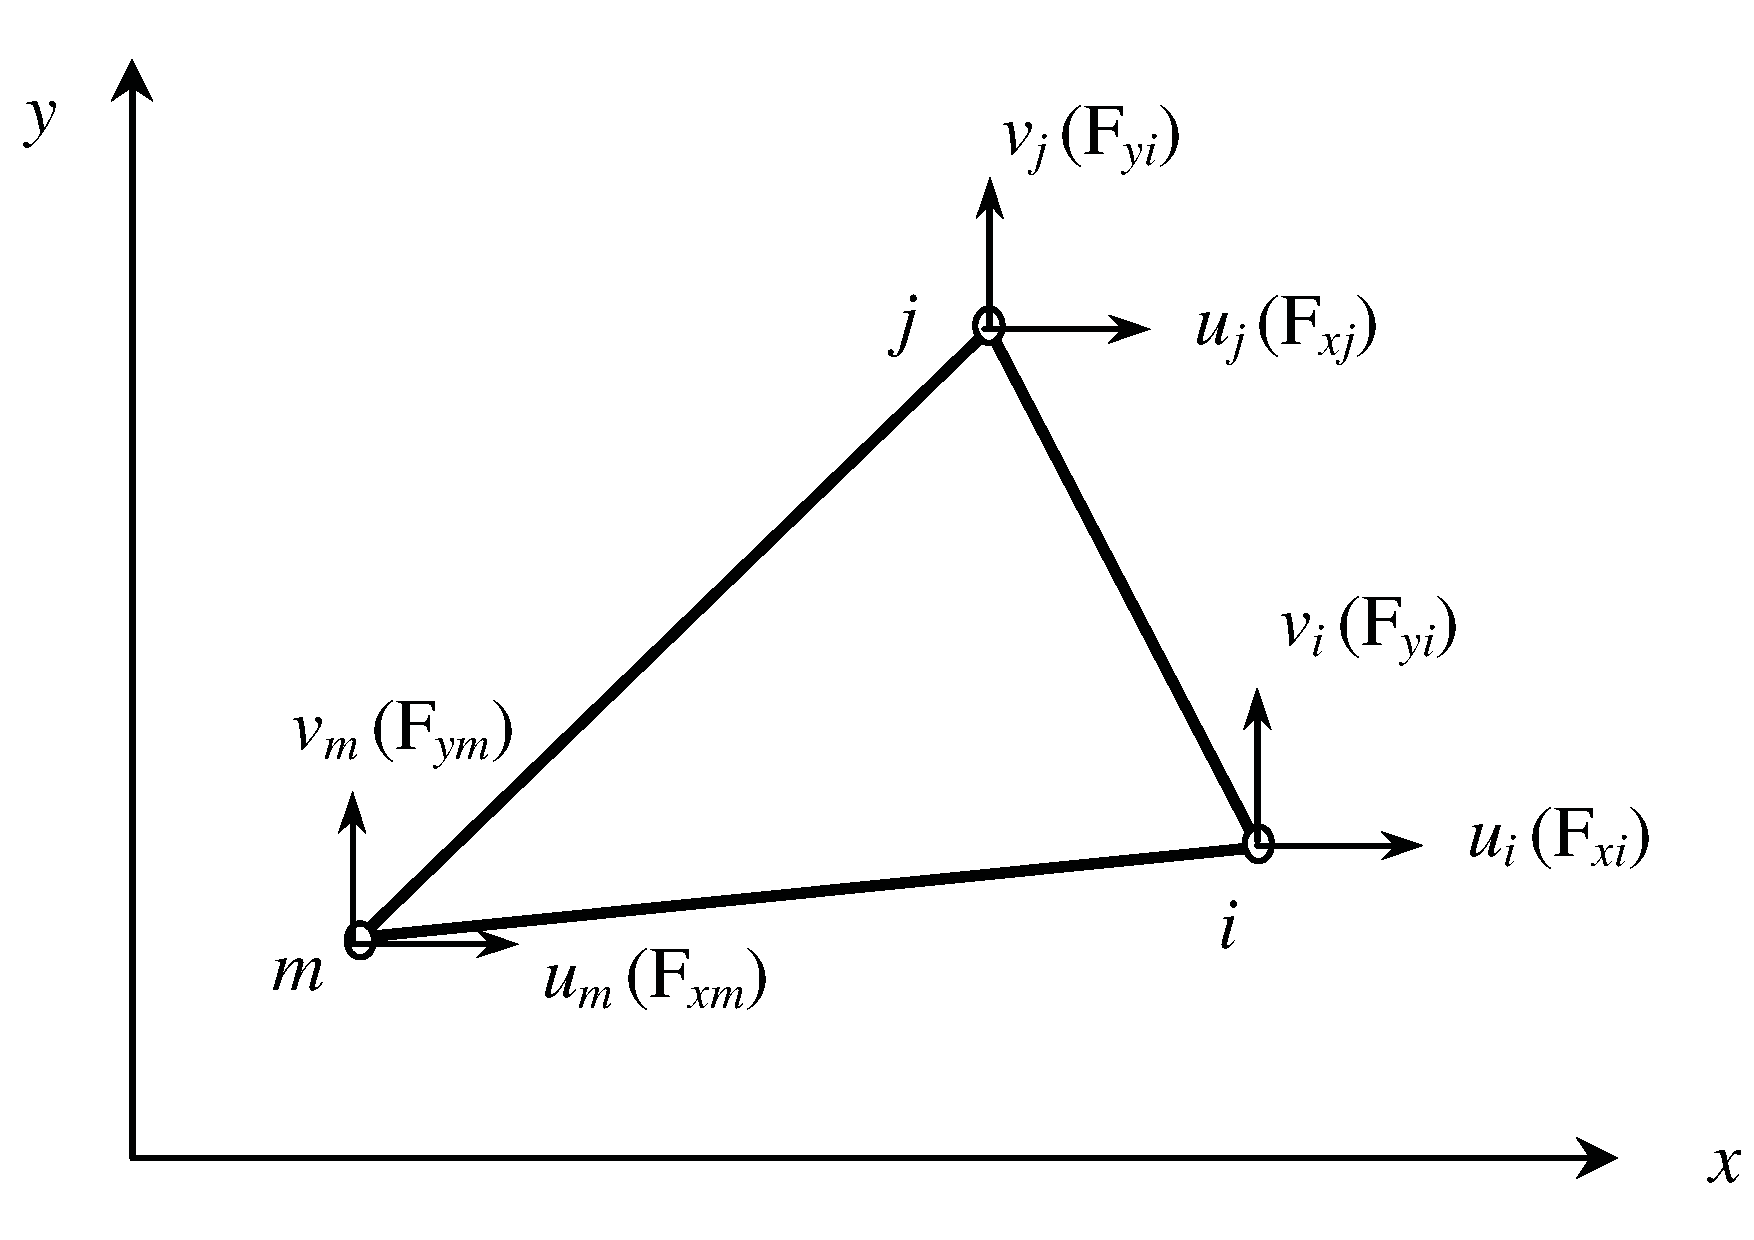
\includegraphics[width=0.5\linewidth]{figure/triangular_membrane_element}
	\caption{Triangular membrane element}
	\label{fig: triangular membrane element}
\end{figure}

By assuming a linear displacement variation inside the element and introducing a set of area coordinates, the displacement model can be expressed as:

\begin{equation} \label{eq: displacement model for CST}
\begin{split}
u &= a_1 + a_2 x + a_3 y \\
v &= a_4 + a_5 x + a_6 y
\end{split}
\end{equation}

By considering the displacements $ u_i $ and $ v_i $ as the local degrees of freedom of node $ i,j,m $, the constants $ a_1, \cdots, a_6 $ can be evaluated. Thus, by using the conditions

\begin{align*}
	u_i &= a_1 + a_2 x_i + a_3 y_i & v_i &= a_4 + a_5 x_i + a_6 y_i \\
	u_j &= a_1 + a_2 x_j + a_3 y_j & v_j &= a_4 + a_5 x_j + a_6 y_j \\
	u_m &= a_1 + a_2 x_m + a_3 y_m & v_m &= a_4 + a_5 x_m + a_6 y_m
\end{align*}

We can express the constants $ a_1, \cdots, a_6 $ in terms of the nodal degrees of freedom:

\begin{align*}
	a_1 &= \frac{1}{2\Delta} 
	\begin{vmatrix}
		u_i & x_i & y_i \\ 
		u_j & x_j & y_j \\ 
		u_m & x_m & y_m
	\end{vmatrix} & a_2 &= \frac{1}{2\Delta} 
	\begin{vmatrix}
		1 & u_i & y_i \\ 
		1 & u_j & y_j \\ 
		1 & u_m & y_m
	\end{vmatrix} & a_3 &= \frac{1}{2\Delta} 
	\begin{vmatrix}
		1 & x_i & u_i \\ 
		1 & x_j & u_j \\ 
		1 & x_m & u_m
	\end{vmatrix} 
\end{align*}

Where 

\begin{equation*}
2\Delta = \begin{vmatrix}
	1 & x_i & y_i \\ 
	1 & x_j & y_j \\ 
	1 & x_m & y_m
\end{vmatrix}
\end{equation*}

This leads to the displacement model:
\begin{align*}
	\vec{U} &= \begin{bmatrix}
		u(x,y) \\
		v(x,y)
	\end{bmatrix} = \begin{bmatrix}
	N
\end{bmatrix} \vec{q}^{(e)} \\
&= \begin{bmatrix}
	N_1(x,y) & 0 & N_2(x,y) & 0 & N_3(x,y) & 0 \\ 
	0 & N_1(x,y) & 0 & N_2(x,y) & 0 & N_3(x,y)
\end{bmatrix} \begin{bmatrix}
u_i \\ 
v_i \\ 
u_j \\ 
v_j \\ 
u_m \\ 
v_m
\end{bmatrix} 
\end{align*}

\begin{align*}
	a_1 &= x_j y_m - x_m y_j & a_2 &= x_m y_i - x_i y_m & a_3 &= x_i y_j - x_j y_i \\
	b_1 &= y_j - y_m & b_2 &= y_m - y_i & b_3 &= y_i - y_j \\
	c_1 &= x_m - x_j & c_2 &= x_i - x_m & c_3 &= x_j - x_i \\
	N_i &= \frac{( a_i + b_i x + c_i y)}{2\Delta} & N_j &= \frac{( a_j + b_j x + c_j y)}{2\Delta} & N_m &= \frac{( a_m + b_m x + c_m y)}{2\Delta}
\end{align*}

\subsection{element Strain}
By using the relations:

\begin{equation}
\mathbf{\epsilon} = \left\lbrace \begin{array}{c}
\epsilon_{xx} \\ 
\epsilon_{yy} \\ 
\epsilon_{xy}
\end{array} \right\rbrace = \left\lbrace \begin{array}{c}
\frac{\partial u}{\partial x} \\ 
\frac{\partial v}{\partial y} \\ 
\frac{\partial u}{\partial y}+\frac{\partial v}{\partial x}
\end{array}  \right\rbrace 
\end{equation}

the components of strain can be expressed in terms of nodal displacements as:

\begin{equation}
\mathbf{\epsilon} = \mathbf{B} \mathbf{q}^{(e)}
\end{equation}

where

\begin{equation}\label{eq: stain matrix}
\mathbf{B} = \frac{1}{2\Delta} \begin{bmatrix}
b_1 & 0 & b_2 & 0 & b_3 & 0 \\ 
0 & c_1 & 0 & c_2 & 0 & c_3 \\ 
c_1 & b_1 & c_2 & b_2 & c_3 & b_3
\end{bmatrix} 
\end{equation}

\subsection{element stress}
The stress-strain relations are given by:

\begin{equation}\label{eq: stress-strain relation of plane stress}
\mathbf{\sigma} = \mathbf{D} \mathbf{\epsilon}
\end{equation}

where

\begin{equation}
\mathbf{\sigma} = \left\lbrace \begin{array}{c}
\sigma_{xx} \\ 
\sigma_{yy} \\ 
\sigma_{xy}
\end{array}  \right\rbrace
\end{equation}

and

\begin{equation}\label{eq: stress-strain relation of plane stress}
\mathbf{D} = \frac{E}{1-\nu^2} \begin{bmatrix}
1 & \nu & 0 \\ 
\nu & 1 & 0 \\ 
0 & 0 & \frac{1-\nu}{2}
\end{bmatrix} 
\end{equation}

\subsection{element stiffness}
the stiffness matrix of the element $ \mathbf{K}_e $ can be found by using:

\begin{equation}\label{eq: membrane element stiffness matrix definition}
\mathbf{K}_e=\iiint_\Omega \mathbf{B}^T \mathbf{DB} d\Omega = \iint_\Delta \mathbf{B}^T \mathbf{DB} h d\Delta
\end{equation}

where $ \Omega $ denotes the volume of the element. If the plate thickness is taken as a constant $ h $, the evaluation of the integral in eq \ref{eq: membrane element stiffness matrix definition} presents no difficult since the elements of the matrices $ \mathbf{B} $ and $ \mathbf{D} $ are all constants (not functions of $ x $ and $ y $). Hence, Eq \ref{eq: membrane element stiffness matrix definition} can be rewritten as:

\begin{equation}\label{eq: memrane element stiffness matrix}
\mathbf{K}_e = \mathbf{B}^T \mathbf{DB} h \iint_\Delta   d\Delta =  h\Delta \mathbf{B}^T \mathbf{DB}
\end{equation}

\section{Discrete Kirchhoff triangle}
A large number of plate t)ending elements tmve beell developed and reported in the literature\todo{references}. In the classical theory of thin plates discussed in this section, certain simplifying approximations are made. One of the important assumptions made is that shear deformation is negligible. Some elements have been developed by including the effect of transverse shear deformation also. \\

According to thin plate theory, the deformation is completely described by the transverse deflection of the middle surface of the plate $ (w) $ only. Thus. if a displacement model is assumed for $ w $. the continuity of not only $ w $ tut also its derivatives has to be maintained between adjacent elements.

\subsection{Displacement model}
\begin{figure}[h!]
\centering
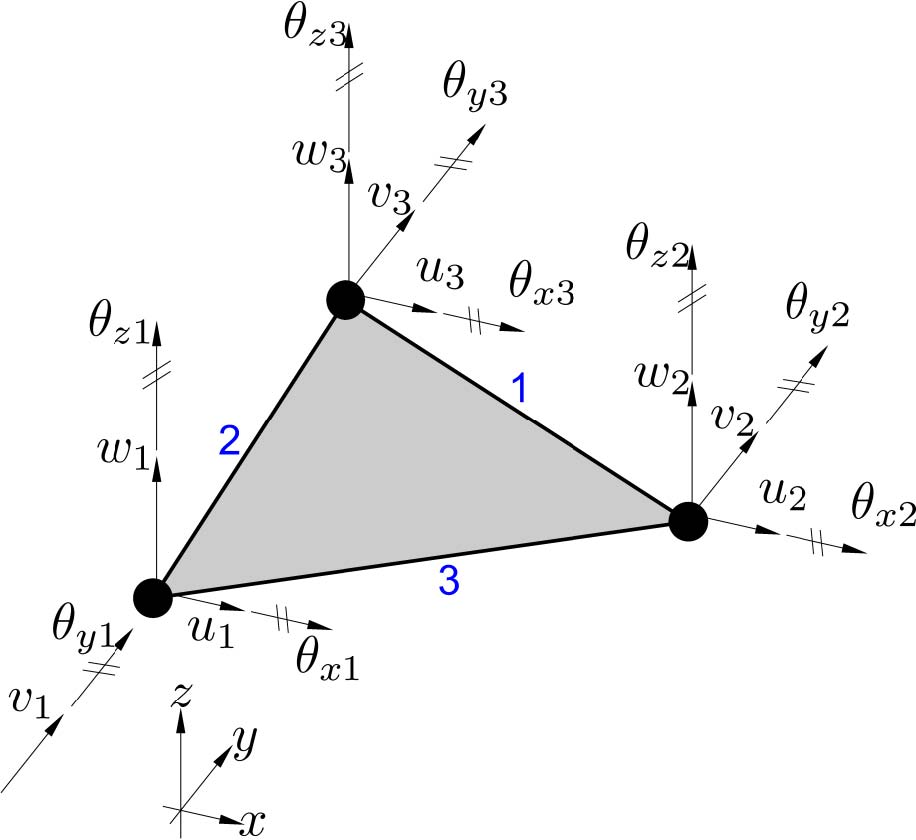
\includegraphics[width=0.5\linewidth]{figure/dofs_of_triangle_element}
\caption{Degrees of freedom of triangle element}
\label{fig: Nodal degrees of freedom of a triangular plate in bending}
\end{figure}

At each node of triangular plate element shown in figure \ref{fig: Nodal degrees of freedom of a triangular plate in bending}. the transverse displacement $ w $ and rotations about the $ x $ and $ y $ axes are taken as the degrees of freedom. Since there are nine displacement degrees of freedom in the element, the assumed polynomial for $ w(x,y) $ must also contain nine constant terms. To maintain geometric isotropy, the displacement model is taken as:

\begin{equation}\label{eq: displacement model for plate bending}
w = a_1 L_1 + a_2 L_2 + a_3 L_3 + a_4 L_2 L_3 + a_5 L_3 L_1 + a_6 L_1 L_2 + a_7 (L_2 L_3^2 - L_3 L_2^2) + a_8 (L_3 L_1^2-L_1 L_3^2) + a_9(L_1 L_2^2 - L_2 L_1^2)
\end{equation}

The first three terms represent rigid displacements and terms 3 \textasciitilde 6 correspond to constant strain. The constants $ (a_1, a_2, \cdots, a_9) $ have to be determined from the nodal conditions:

substitute area coordinates of nodes into eq \ref{eq: displacement model for plate bending}, we have:

\begin{equation} \label{eq: constant terms 1-3}
a_1 = w_1~~~~a_2 = w_2~~~~a_3 = w_3
\end{equation}

By computing derivatives of deflection w to area coordinates:

\begin{equation} \label{eq: derivatives of deflection to area coordinates for plate bending}
\begin{split}
\frac{\partial w}{\partial L_1}	&= w_1 - w_3 - a_4 L_2 + a_5 (L_3-L_1) + a_6 L_2 + a_7(L_2^2-2L_2L_3) + a_8(4L_1 L_3 - L_1^2 - L_3^2) + a_9(L_2^2 - 2L_1 L_2) \\
\frac{\partial w}{\partial L_2}	&= w_2 - w_3 + a_4 (L_3-L_2) - a_5 L_1 + a_6 L_1 + a_7(L_3^2 + L_2^2 - 4L_2 L_3) + a_8(2L_1 L_3 - L_1^2) + a_9(2L_1 L_2 - L_1^2)
\end{split}
\end{equation}

In the equation, $ w_{,L_{ij}} $ means derivative of deflection $ w $ to area coordinate $ L_i $ at node $ j $. The constants can be solved:

\begin{equation} \label{eq: constant terms 4-9}
\begin{split}
a_4 &= \frac{w_{,L_{23}} - w_{,L_{22}}}{2} \\
a_5 &= \frac{w_{,L_{13}} - w_{,L_{11}}}{2} \\
a_6 &= \frac{w_{,L_{12}} + w_{,L_{21}} - w_{,L_{11}} - w_{,L_{22}}}{2} \\
a_7 &= w_3 - w_2 + \frac{w_{,L_{23}} + w_{,L_{22}}}{2} \\
a_8 &= w_1 - w_3 - \frac{w_{,L_{11}} + w_{,L_{13}}}{2} \\
a_9 &= w_2 - w_1 + \frac{w_{,L_{11}} + w_{,L_{12}} - w_{,L_{21}} - w_{,L_{22}}}{2}
\end{split}
\end{equation}

Note the $ L_3 $ is not a dependent variable, it should be regarded as $ 1-L_1 - L_2 $. substitue area coordinates of three nodes into equation \ref{eq: derivatives of deflection to area coordinates for plate bending}, we get:

\begin{align*}
	w_{,L_{11}} &= w_1 - w_3 - a_5 -a_8 & w_{,L_{21}} &= w_2 - w_3 - a_5 + a_6 -a_8 -a_9 \\
	w_{,L_{12}} &= w_1 - w_3 -a_4 + a_6 + a_7 + a_9 & w_{,L_{22}} &= w_2- w_3-a_4+a_7 \\
	w_{,L_{13}} &= w_1 - w_3 + a_5 -a_8 & w_{,L_{23}} &= w_2 - w_3 + a_4 + a_7
\end{align*}

substitute eq \ref{eq: constant terms 1-3} and \ref{eq: constant terms 4-9} into eq \ref{eq: displacement model for plate bending}, it gives:

\begin{equation} \label{eq: nodal displacements definition}
w = \begin{bmatrix}
\bar{\mathbf{N}}_i & \bar{\mathbf{N}}_j & \bar{\mathbf{N}}_m
\end{bmatrix}
 \begin{bmatrix}
 \bar{\mathbf{\delta}}_i \\ 
 \bar{\mathbf{\delta}}_j \\ 
 \bar{\mathbf{\delta}}_m
 \end{bmatrix} 
\end{equation}

where:

\begin{equation*}
	\begin{split}
	\bar{\mathbf{\delta}}_1 = \begin{bmatrix}
		w_1 & w_{,L_{11}} & w_{,L_{21}}
		\end{bmatrix}~~~~\bar{\mathbf{\delta}}_2 = \begin{bmatrix}
		w_2 & w_{,L_{12}} & w_{,L_{21}} \end{bmatrix}~~~~\bar{\mathbf{\delta}}_3 = \begin{bmatrix}	w_3 & w_{,L_{13}} & w_{,L_{23}} \end{bmatrix} \\
		\bar{\mathbf{N}}_1 = \begin{bmatrix}
			N_1 & N_{,L_{11}} & N_{,L_{21}}
		\end{bmatrix}~~~~\bar{\mathbf{N}}_2 = \begin{bmatrix}
		N_2 & N_{,L_{12}} & N_{,L_{21}} \end{bmatrix}~~~~\bar{\mathbf{N}}_3 = \begin{bmatrix}	N_3 & N_{,L_{13}} & N_{,L_{23}} \end{bmatrix}
	\end{split}	
\end{equation*}

the components of the shape function are:

\begin{align*}
	N_1 &= L_1 -(L_1 L_2^2 - L_2 L_1^2) + (L_3 L_1^2 - L_1 L_3^2) \\
	N_{L_{11}} &= \frac{-L_1 L_2 - L_3 L_1 + (L_1 L_2^2 - L_2 L_1^2) - (L_3 L_1^2 - L_1 L_3^2)}{2} \\
	N_{L_{21}} &= \frac{L_1 L_2 + (L_2 L_1^2 - L_1 L_2^2)}{2} \\
	N_{2} &= L_2 -(L_2 L_3^2-L_3 L_2^2) + (L_1 L_2^2 -L_2 L_1^2) \\
	N_{L_{12}} &= \frac{L_1 L_2 + (L_1 L_2^2 - L_2 L_1^2)}{2} \\
	N_{L_{22}} &= \frac{-L_2 L_3 - L_1 L_2 +(L_2 L_3^2-L_3 L_2^2)- (L_1 L_2^2 - L_2 L_1^2)}{2} \\
	N_3 &= L_3 - (L_3 L_1^2 -L_1 L_3^2) + (L_2 L_3^2 - L_3 L_2^2) \\
	N_{L_{13}} &= \frac{L_1 L_3 + (L_1 L_3^2 - L_3 L_i^2)}{2} \\
	N_{L_{23}} &= \frac{L_2 L_3 + (L_2 L_3^2 - L_3 L_2^2)}{2}
\end{align*}

as we have:

\begin{equation}
\begin{split}
\frac{\partial x}{\partial L_1} &= x_1 - x_3 = c_1 \\
\frac{\partial y}{\partial L_1} &= y_1 - y_3 = -b_1 \\
\frac{\partial x}{\partial L_2} &= x_2 - x_3 = -c_1 \\
\frac{\partial y}{\partial L_2} &= x_2 - x_3 = b_1
\end{split}
\end{equation}

this leads to

\begin{equation}\label{key}
\begin{split}
\frac{\partial w}{\partial L_1} = c_2 \frac{\partial w}{\partial x} - b_2 \frac{\partial w}{\partial y} = -b_2 \theta_x - c_2 \theta_y \\
\frac{\partial w}{\partial L_2} = -c_2 \frac{\partial w}{\partial x} + b_2 \frac{\partial w}{\partial y} = b_2 \theta_x + c_2 \theta_y \\
\end{split}
\end{equation}

The relation of nodal displacements between cardisian system and area system is:

\begin{equation}\label{eq: cardisian to area coordinates transform.}
\bar{\mathbf{\delta}}_i = \begin{bmatrix}
w_i \\ 
w_{,L_{11}} \\ 
w_{,L_{21}}
\end{bmatrix} = \begin{bmatrix}
1 & 0 & 0 \\ 
0 & -b_2 & -c_2 \\ 
0 & b_1 & c_1
\end{bmatrix} \begin{bmatrix}
w_i \\ 
\theta_{xi} \\ 
\theta_{yi}
\end{bmatrix} = \mathbf{P} \mathbf{\delta}_i
\end{equation}

Use eq \ref{eq: cardisian to area coordinates transform.}, the eq \ref{eq: nodal displacements definition} can be re-written as:

\begin{equation}\label{key}
w = \begin{bmatrix}
\bar{\mathbf{N}}_1 & \bar{\mathbf{N}}_2 & \bar{\mathbf{N}}_3
\end{bmatrix} \begin{bmatrix}
\mathbf{P} & \mathbf{0} & \mathbf{0} \\ 
\mathbf{0} & \mathbf{P} & \mathbf{0} \\ 
\mathbf{0} & \mathbf{0} & \mathbf{P}
\end{bmatrix} \begin{bmatrix}
\mathbf{\delta}_1 \\ 
\mathbf{\delta}_2 \\ 
\mathbf{\delta}_3
\end{bmatrix} = \begin{bmatrix}
\mathbf{N}_1 & \mathbf{N}_2 & \mathbf{N}_3
\end{bmatrix} \begin{bmatrix}
\mathbf{\delta}_1 \\ 
\mathbf{\delta}_2 \\ 
\mathbf{\delta}_3
\end{bmatrix}
\end{equation}

where

\begin{align*}\label{eq: shape function in area coordinates for bending plate}
\mathbf{N}_i &= \bar{\mathbf{N}}_i \mathbf{P} = \begin{bmatrix}
N_i & N_{xi} & N_{yi}
\end{bmatrix}\\
N_i &= L_i + L_i^2 L_j + L_i^2 L_m - L_i L_j^2 - L_i L_m^2  ~~~~~(i=1,2,3) \\
N_{xi} &= b_j L_i^2 L_m - b_m L_i^2 L_j + \frac{(b_j-b_m)}{2}L_i L_j L_m \\
N_{yi} &= c_j L_i^2 L_m - c_m L_i^2 L_j + \frac{c_j - c_m}{2} L_i L_j L_m
\end{align*}

\subsection{Stiffness matrix}
In eq \ref{eq: shape function for bending plate}, the shape function is using $ L_1 $ and $ L_2 $ as independent variables. To obtain stiffness matrix in global space, transformation matrix is introduced:

\begin{equation}\label{key}
\begin{bmatrix}
\partial / \partial x \\ 
\partial / \partial y
\end{bmatrix} = \frac{1}{2\Delta} \begin{bmatrix}
b_1 & b_2 \\ 
c_1 & c_2
\end{bmatrix} \begin{bmatrix}
\partial / \partial L_1 \\ 
\partial / \partial L_2
\end{bmatrix} 
\end{equation}

 and 
 
 \begin{equation}\label{key}
 \begin{bmatrix}
 \partial^2 / \partial x^2 \\ 
 \partial^2 / \partial y^2 \\
2 \partial^2 / \partial x \partial y
 \end{bmatrix} = \frac{1}{4\Delta^2} \mathbf{T} \begin{bmatrix}
 \partial^2 / \partial L_1^2 \\ 
 \partial^2 / \partial L_2^2 \\
 \partial^2 / \partial L_1 \partial L_2
 \end{bmatrix} 
 \end{equation}

where

\begin{equation}\label{key}
\mathbf{T} = \begin{bmatrix}
b_1^2 & b_2^2 & 2 b_1 b_2 \\ 
c_1^2 & c_2^2 & 2 c_1 c_2 \\ 
2 b_1 c_1 & 2 b_2 c_2 & 2 ( b_1 c_2 + b_2 c_1)
\end{bmatrix} 
\end{equation}

the element strain matrix is now:

\begin{equation}\label{key}
\mathbf{\epsilon} = \mathbf{B} \mathbf{\delta^e} = z \begin{bmatrix}
\mathbf{B}_i & \mathbf{B}_j & \mathbf{B}_m
\end{bmatrix} \begin{bmatrix}
\mathbf{\delta}_i \\ 
\mathbf{\delta}_j \\ 
\mathbf{\delta}_m
\end{bmatrix} 
\end{equation}

where

\begin{equation}\label{key}
\mathbf{B}_k = -\begin{bmatrix}
\mathbf{N}_{k,xx} \\ 
\mathbf{N}_{k,yy} \\ 
\mathbf{N}_{k,xy}
\end{bmatrix} = - \frac{1}{4 \Delta^2} \mathbf{T} \begin{bmatrix}
\mathbf{N}_{k,11} \\ 
\mathbf{N}_{k,22} \\ 
\mathbf{N}_{k,12}
\end{bmatrix}~~~~ (k=1,2,3)
\end{equation}

and the element stiffness matrix  \todo{h3 / 12} in global space is:

\begin{equation}\label{eq: gauss quadrature for triangular domain}
\mathbf{K}^e = \frac{h^3}{12} \iint_\Omega \mathbf{B}^T \mathbf{DB} dx dy
\end{equation}

In eq \ref{eq: gauss quadrature for triangular domain}, $ n $ is number of gauss points, $ W_i $ is weight, $ (L_{i1}, L_{i2}, L_{i3}) $ is integration point.

\subsection{Gauss quadrature}
To simplify computation, we use quadrature for solving stiffness integral:

Firstly, the integral over triangular domain $ \Omega $ is converted to:

\begin{equation}\label{key}
\iint_\Omega f(L_1, L_2, L_3) dx dy = 2 \Delta \int_{0}^{1} \int_{0}^{1-L_1} f(L_1, L_2, L_3) dL_1 dL_2
\end{equation}

the right term can be calcultated using:

\begin{equation}\label{key}
\int_{0}^{1} \int_{0}^{1-L_1} f(L_1, L_2, L_3) dL_1 dL_2 = \sum_{i=1}^{n} W_i f(L_{i1}, L_{i2}, L_{i3})
\end{equation}

\begin{figure}[h!]
\centering
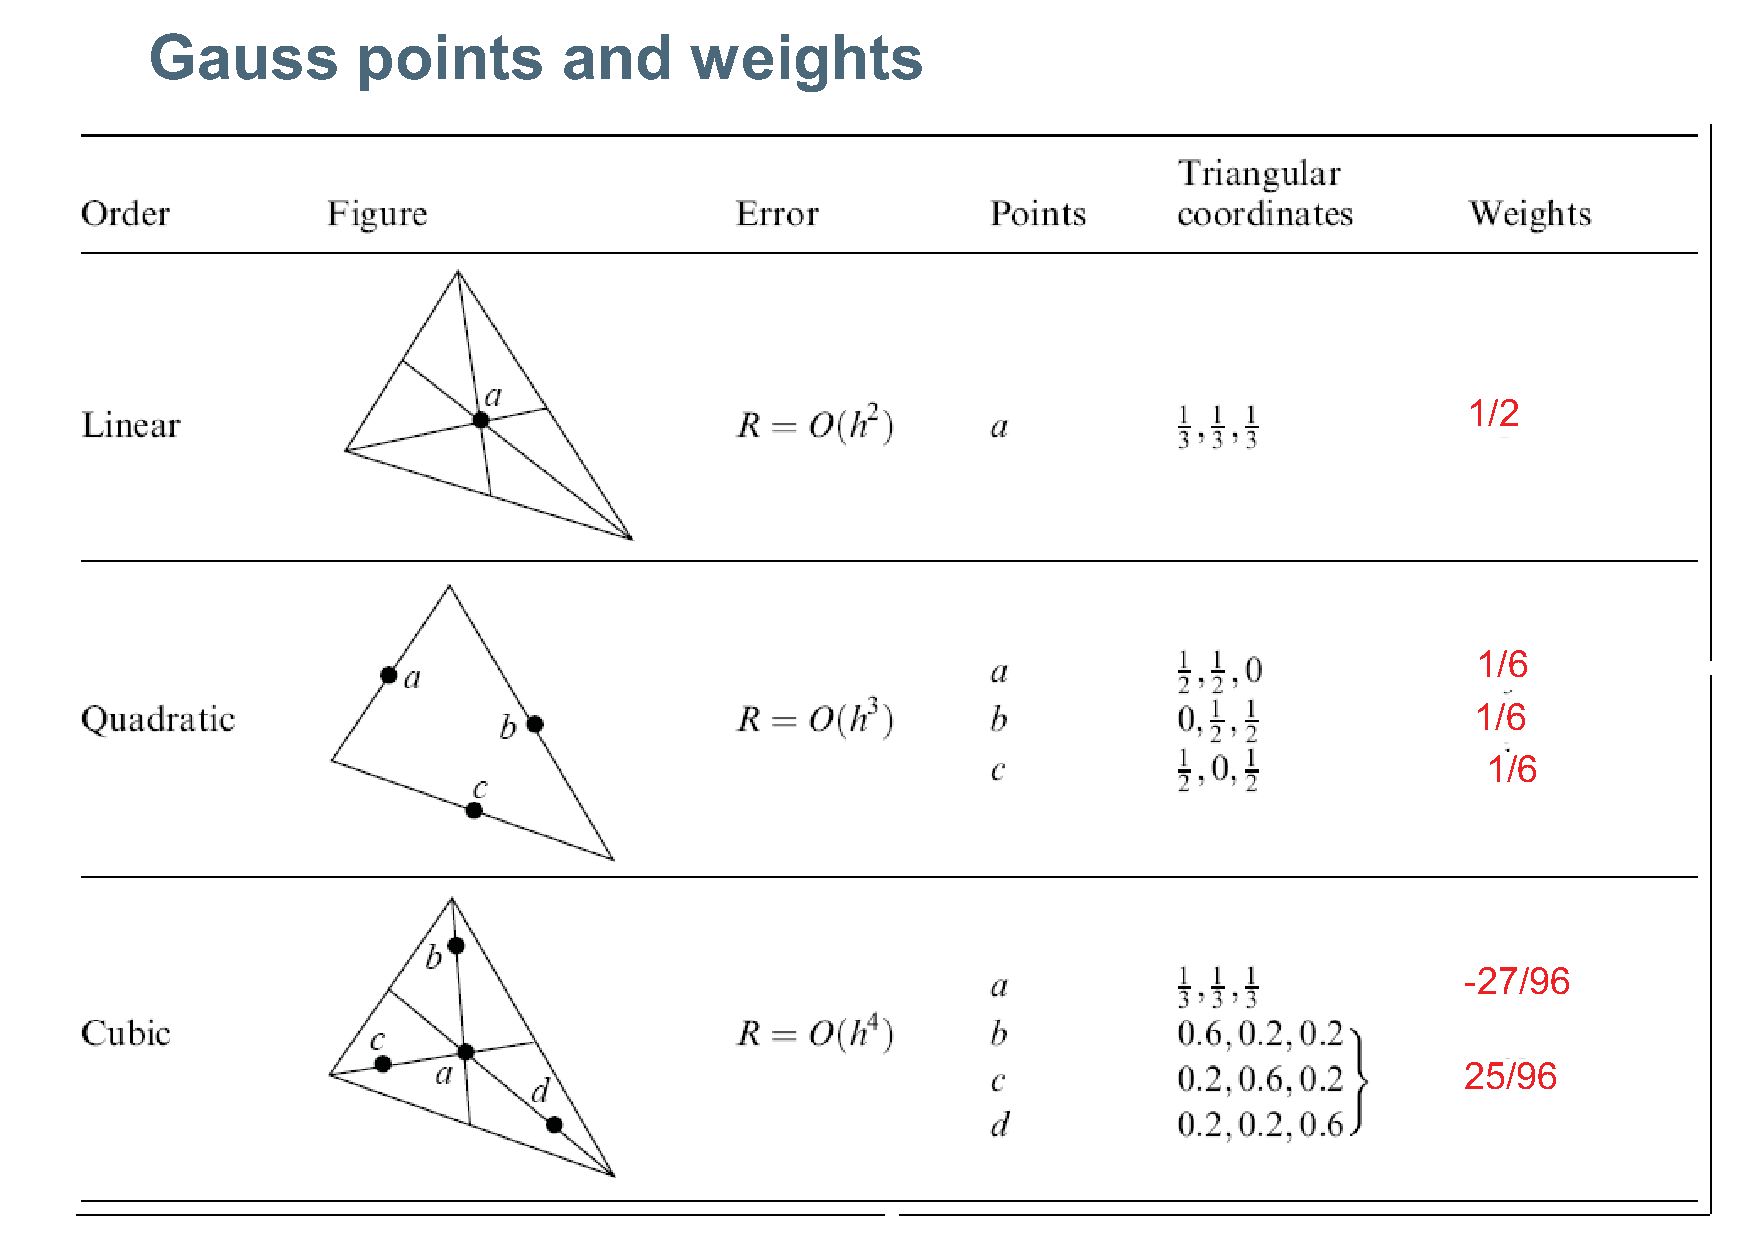
\includegraphics[width=0.4\linewidth]{figure/gauss_points_and_weights}
\caption{gauss points and weights}
\label{fig: gauss points and weights}
\end{figure}

\section{Drilling degree. to be added}

\section{Transformation Matrix}
The shape functions are defined in the plane of the triangle, i.e. z-coordinates for the nodes are equal to zero

\begin{figure}[h!]
	\centering
	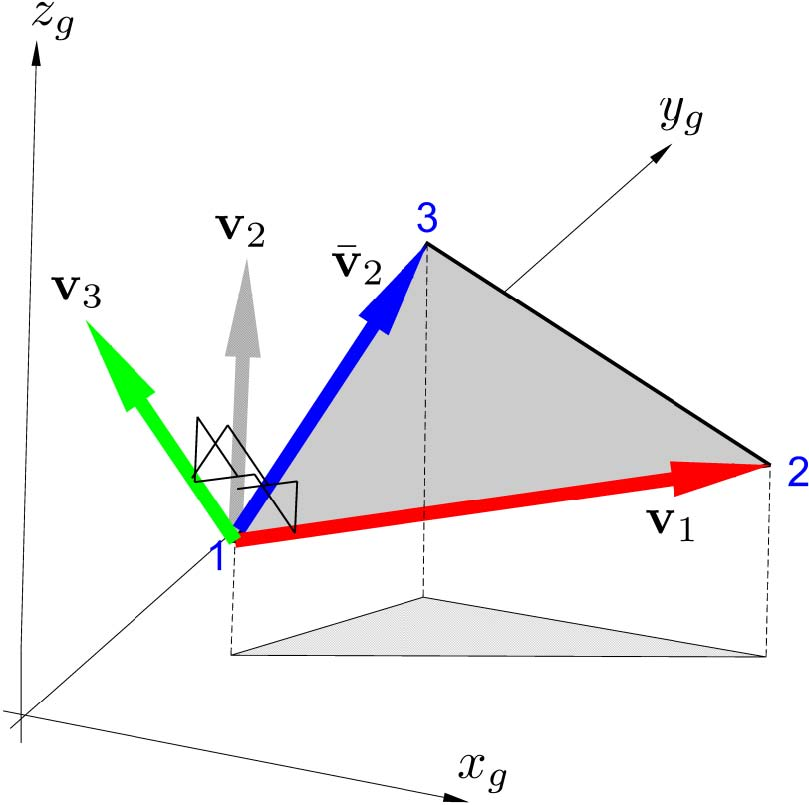
\includegraphics[width=0.5\linewidth]{figure/transformation_matrix}
	\caption{transformation matrix in 3d}
	\label{fig:transformationmatrix}
\end{figure}

Assuming that the triangular element under consideration is an interior element of a large structure. let the node numbers 1, 2, and 3 of the element correspond to the node numbers i, j. and
k, respectively, of the global system. Then place the origin of the local xg system at node 1 (node i), and take the y axis along the edge 1 2 (edge ij) and the x axis perpendicular
to the y axis directed toward node 3 (node k) as shown in Figure \ref{fig: unit vectors for transformation}.

\begin{figure}[h!]
\centering
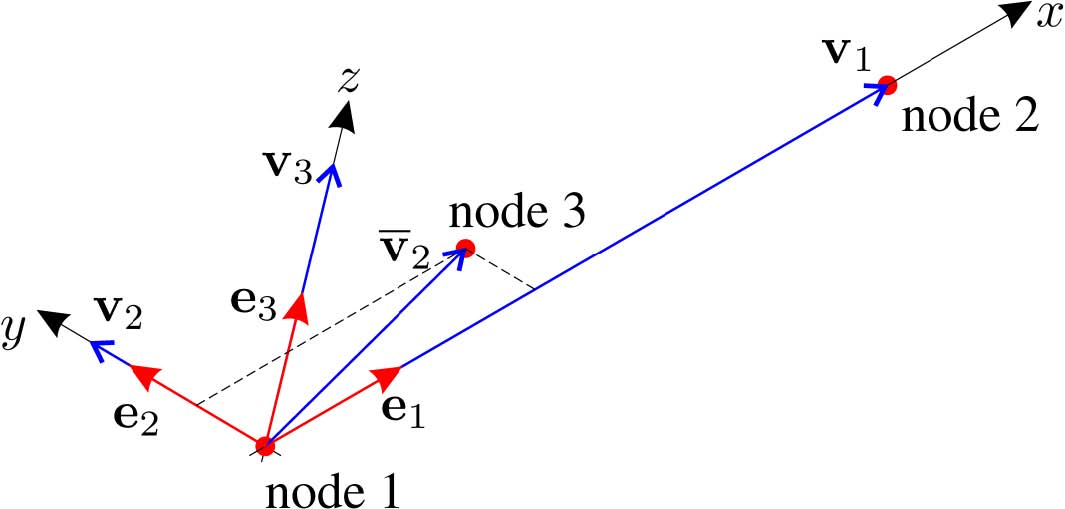
\includegraphics[width=0.5\linewidth]{figure/unit_vectors_for_transformation}
\caption{unit vectors describing xyz sysem.}
\label{fig: unit vectors for transformation}
\end{figure}

We have:

\begin{align*}
	\mathbf{v}_1 &= \begin{bmatrix}
		x_2-x_1 \\ 
		y_2-y_1 \\ 
		z_2-z_1
		\end{bmatrix} \\
		 \bar{\mathbf{v}}_2 &= \begin{bmatrix}
		x_3-x_1 \\ 
		y_3-y_1 \\ 
		z_3-z_1 
	\end{bmatrix} \\
	 \mathbf{v}_3 &= \mathbf{v}_1 \times \bar{\mathbf{v}}_2 \\
	 \mathbf{v}_2 &= \mathbf{v}_3 \times \mathbf{v}_1
\end{align*}

the unit vectors can be expressed:

\begin{align*}
	\mathbf{e}_1 &= \frac{\mathbf{v}_1}{|\mathbf{v}_1|} \\
	\mathbf{e}_2 &= \frac{\mathbf{v}_2}{|\mathbf{v}_2|} \\
	\mathbf{e}_3 &= \frac{\mathbf{v}_3}{|\mathbf{v}_3|}
\end{align*}

So the transformation matrix is:

\begin{equation}
\mathbf{T} = \begin{bmatrix}
\mathbf{e}_1 & \mathbf{e}_2 & \mathbf{e}_3
\end{bmatrix} 
\end{equation}

\begin{equation}
\begin{bmatrix}
x_l \\ 
y_l \\ 
z_l
\end{bmatrix} = \mathbf{T}^T \begin{bmatrix}
x_g \\ 
y_g \\ 
z_g
\end{bmatrix} 
\end{equation}

\section{global element stiffness matrix}
The full transformation matrix $ (12x12) $ can be made from $ T (3x3) $ and multiply the local element stiffness matrix with the transformation to obtain the global element stiffness matrix:

\begin{equation}\label{eq: full transformation matrix for plate.}
\mathbf{T}_g = \begin{bmatrix}
\mathbf{T} & \mathbf{0} & \mathbf{0} \\ 
\mathbf{0} & \mathbf{T} & \mathbf{0} \\ 
\mathbf{0} & \mathbf{0} & \mathbf{T}
\end{bmatrix} 
\end{equation}

\begin{equation}\label{eq: gobal element stiffness matrix}
\mathbf{K}_{eg} = \mathbf{T}_g \mathbf{K}_e \mathbf{T}_g^T
\end{equation}